% Auto-generated by tools/paper_race_tikz.py -- lift the tikzpicture into your IEEE paper,
% or compile this file directly (pdflatex/lualatex). Needs pgfplots >= 1.16.
\documentclass[tikz,border=2pt]{standalone}
\usepackage{pgfplots}
\pgfplotsset{compat=1.18}
\usepgfplotslibrary{groupplots,colormaps}
\definecolor{cstatic}{RGB}{153,153,153}
\definecolor{cslower}{RGB}{0,114,178}
\definecolor{cequal}{RGB}{0,158,115}
\definecolor{cfaster}{RGB}{213,94,0}
\begin{document}
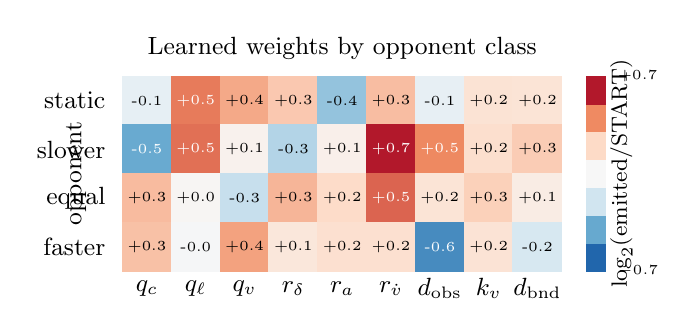
\begin{tikzpicture}[rgb color/.style={/utils/exec={\definecolor{tmpc}{RGB}{#1}}, draw=tmpc, fill=tmpc}, x=0.62cm, y=0.62cm]
\fill[rgb color={230,239,244}] (0,3) rectangle (1,4);
\node[font=\tiny, black] at (0.5,3.5) {-0.1};
\fill[rgb color={231,123,91}] (1,3) rectangle (2,4);
\node[font=\tiny, white] at (1.5,3.5) {+0.5};
\fill[rgb color={244,169,136}] (2,3) rectangle (3,4);
\node[font=\tiny, black] at (2.5,3.5) {+0.4};
\fill[rgb color={250,200,176}] (3,3) rectangle (4,4);
\node[font=\tiny, black] at (3.5,3.5) {+0.3};
\fill[rgb color={148,195,221}] (4,3) rectangle (5,4);
\node[font=\tiny, black] at (4.5,3.5) {-0.4};
\fill[rgb color={248,189,162}] (5,3) rectangle (6,4);
\node[font=\tiny, black] at (5.5,3.5) {+0.3};
\fill[rgb color={231,239,244}] (6,3) rectangle (7,4);
\node[font=\tiny, black] at (6.5,3.5) {-0.1};
\fill[rgb color={251,227,212}] (7,3) rectangle (8,4);
\node[font=\tiny, black] at (7.5,3.5) {+0.2};
\fill[rgb color={251,228,214}] (8,3) rectangle (9,4);
\node[font=\tiny, black] at (8.5,3.5) {+0.2};
\fill[rgb color={105,170,208}] (0,2) rectangle (1,3);
\node[font=\tiny, white] at (0.5,2.5) {-0.5};
\fill[rgb color={225,112,85}] (1,2) rectangle (2,3);
\node[font=\tiny, white] at (1.5,2.5) {+0.5};
\fill[rgb color={248,241,237}] (2,2) rectangle (3,3);
\node[font=\tiny, black] at (2.5,2.5) {+0.1};
\fill[rgb color={179,212,231}] (3,2) rectangle (4,3);
\node[font=\tiny, black] at (3.5,2.5) {-0.3};
\fill[rgb color={249,239,234}] (4,2) rectangle (5,3);
\node[font=\tiny, black] at (4.5,2.5) {+0.1};
\fill[rgb color={178,24,43}] (5,2) rectangle (6,3);
\node[font=\tiny, white] at (5.5,2.5) {+0.7};
\fill[rgb color={238,137,97}] (6,2) rectangle (7,3);
\node[font=\tiny, white] at (6.5,2.5) {+0.5};
\fill[rgb color={252,223,206}] (7,2) rectangle (8,3);
\node[font=\tiny, black] at (7.5,2.5) {+0.2};
\fill[rgb color={250,204,181}] (8,2) rectangle (9,3);
\node[font=\tiny, black] at (8.5,2.5) {+0.3};
\fill[rgb color={248,187,159}] (0,1) rectangle (1,2);
\node[font=\tiny, black] at (0.5,1.5) {+0.3};
\fill[rgb color={247,245,243}] (1,1) rectangle (2,2);
\node[font=\tiny, black] at (1.5,1.5) {+0.0};
\fill[rgb color={199,223,237}] (2,1) rectangle (3,2);
\node[font=\tiny, black] at (2.5,1.5) {-0.3};
\fill[rgb color={246,181,152}] (3,1) rectangle (4,2);
\node[font=\tiny, black] at (3.5,1.5) {+0.3};
\fill[rgb color={253,220,201}] (4,1) rectangle (5,2);
\node[font=\tiny, black] at (4.5,1.5) {+0.2};
\fill[rgb color={219,100,80}] (5,1) rectangle (6,2);
\node[font=\tiny, white] at (5.5,1.5) {+0.5};
\fill[rgb color={251,228,214}] (6,1) rectangle (7,2);
\node[font=\tiny, black] at (6.5,1.5) {+0.2};
\fill[rgb color={251,209,186}] (7,1) rectangle (8,2);
\node[font=\tiny, black] at (7.5,1.5) {+0.3};
\fill[rgb color={249,236,228}] (8,1) rectangle (9,2);
\node[font=\tiny, black] at (8.5,1.5) {+0.1};
\fill[rgb color={248,193,166}] (0,0) rectangle (1,1);
\node[font=\tiny, black] at (0.5,0.5) {+0.3};
\fill[rgb color={245,246,247}] (1,0) rectangle (2,1);
\node[font=\tiny, black] at (1.5,0.5) {-0.0};
\fill[rgb color={243,162,127}] (2,0) rectangle (3,1);
\node[font=\tiny, black] at (2.5,0.5) {+0.4};
\fill[rgb color={250,231,219}] (3,0) rectangle (4,1);
\node[font=\tiny, black] at (3.5,0.5) {+0.1};
\fill[rgb color={252,224,208}] (4,0) rectangle (5,1);
\node[font=\tiny, black] at (4.5,0.5) {+0.2};
\fill[rgb color={252,224,208}] (5,0) rectangle (6,1);
\node[font=\tiny, black] at (5.5,0.5) {+0.2};
\fill[rgb color={71,139,191}] (6,0) rectangle (7,1);
\node[font=\tiny, white] at (6.5,0.5) {-0.6};
\fill[rgb color={251,227,213}] (7,0) rectangle (8,1);
\node[font=\tiny, black] at (7.5,0.5) {+0.2};
\fill[rgb color={215,232,241}] (8,0) rectangle (9,1);
\node[font=\tiny, black] at (8.5,0.5) {-0.2};
\node[font=\small] at (0.5,-0.35) {$q_c$};
\node[font=\small] at (1.5,-0.35) {$q_\ell$};
\node[font=\small] at (2.5,-0.35) {$q_v$};
\node[font=\small] at (3.5,-0.35) {$r_\delta$};
\node[font=\small] at (4.5,-0.35) {$r_a$};
\node[font=\small] at (5.5,-0.35) {$r_{\dot v}$};
\node[font=\small] at (6.5,-0.35) {$d_\mathrm{obs}$};
\node[font=\small] at (7.5,-0.35) {$k_v$};
\node[font=\small] at (8.5,-0.35) {$d_\mathrm{bnd}$};
\node[font=\small, anchor=east] at (-0.15,3.5) {static};
\node[font=\small, anchor=east] at (-0.15,2.5) {slower};
\node[font=\small, anchor=east] at (-0.15,1.5) {equal};
\node[font=\small, anchor=east] at (-0.15,0.5) {faster};
\node[font=\small, rotate=90] at (-0.95,2.0) {opponent};
\fill[rgb color={33,102,172}] (9.5,0.000) rectangle (9.9,0.571);
\fill[rgb color={103,169,207}] (9.5,0.571) rectangle (9.9,1.143);
\fill[rgb color={209,229,240}] (9.5,1.143) rectangle (9.9,1.714);
\fill[rgb color={247,247,247}] (9.5,1.714) rectangle (9.9,2.286);
\fill[rgb color={253,219,199}] (9.5,2.286) rectangle (9.9,2.857);
\fill[rgb color={239,138,98}] (9.5,2.857) rectangle (9.9,3.429);
\fill[rgb color={178,24,43}] (9.5,3.429) rectangle (9.9,4.000);
\node[font=\tiny, anchor=west] at (9.95,4) {$+0.7$};
\node[font=\tiny, anchor=west] at (9.95,0) {$-0.7$};
\node[font=\footnotesize, anchor=south, rotate=90] at (10.65,2.0) {$\log_2(\mathrm{emitted}/\mathrm{START})$};
\node[font=\small, anchor=south] at (4.5,4.15) {Learned weights by opponent class};
\end{tikzpicture}
\end{document}
